\section{Results}

\subsection{The theoretical models}

\begin{figure}[H]
    \centering    
    
\includegraphics[height=0.37\textwidth]{Figures/2layer_angle.png}
    \caption{Surface angle as a function of the dimensionless layer thickness $\varphi = H/h_1$ for the two-layer viscosity model. Different curves correspond to different viscosity ratios $\epsilon = h_2/h_1$. The classical Ekman angle of $45^\circ$ is shown as a reference.}
    \label{fig:2layer_angle}
\end{figure}

\begin{figure}[H]
    \centering    
    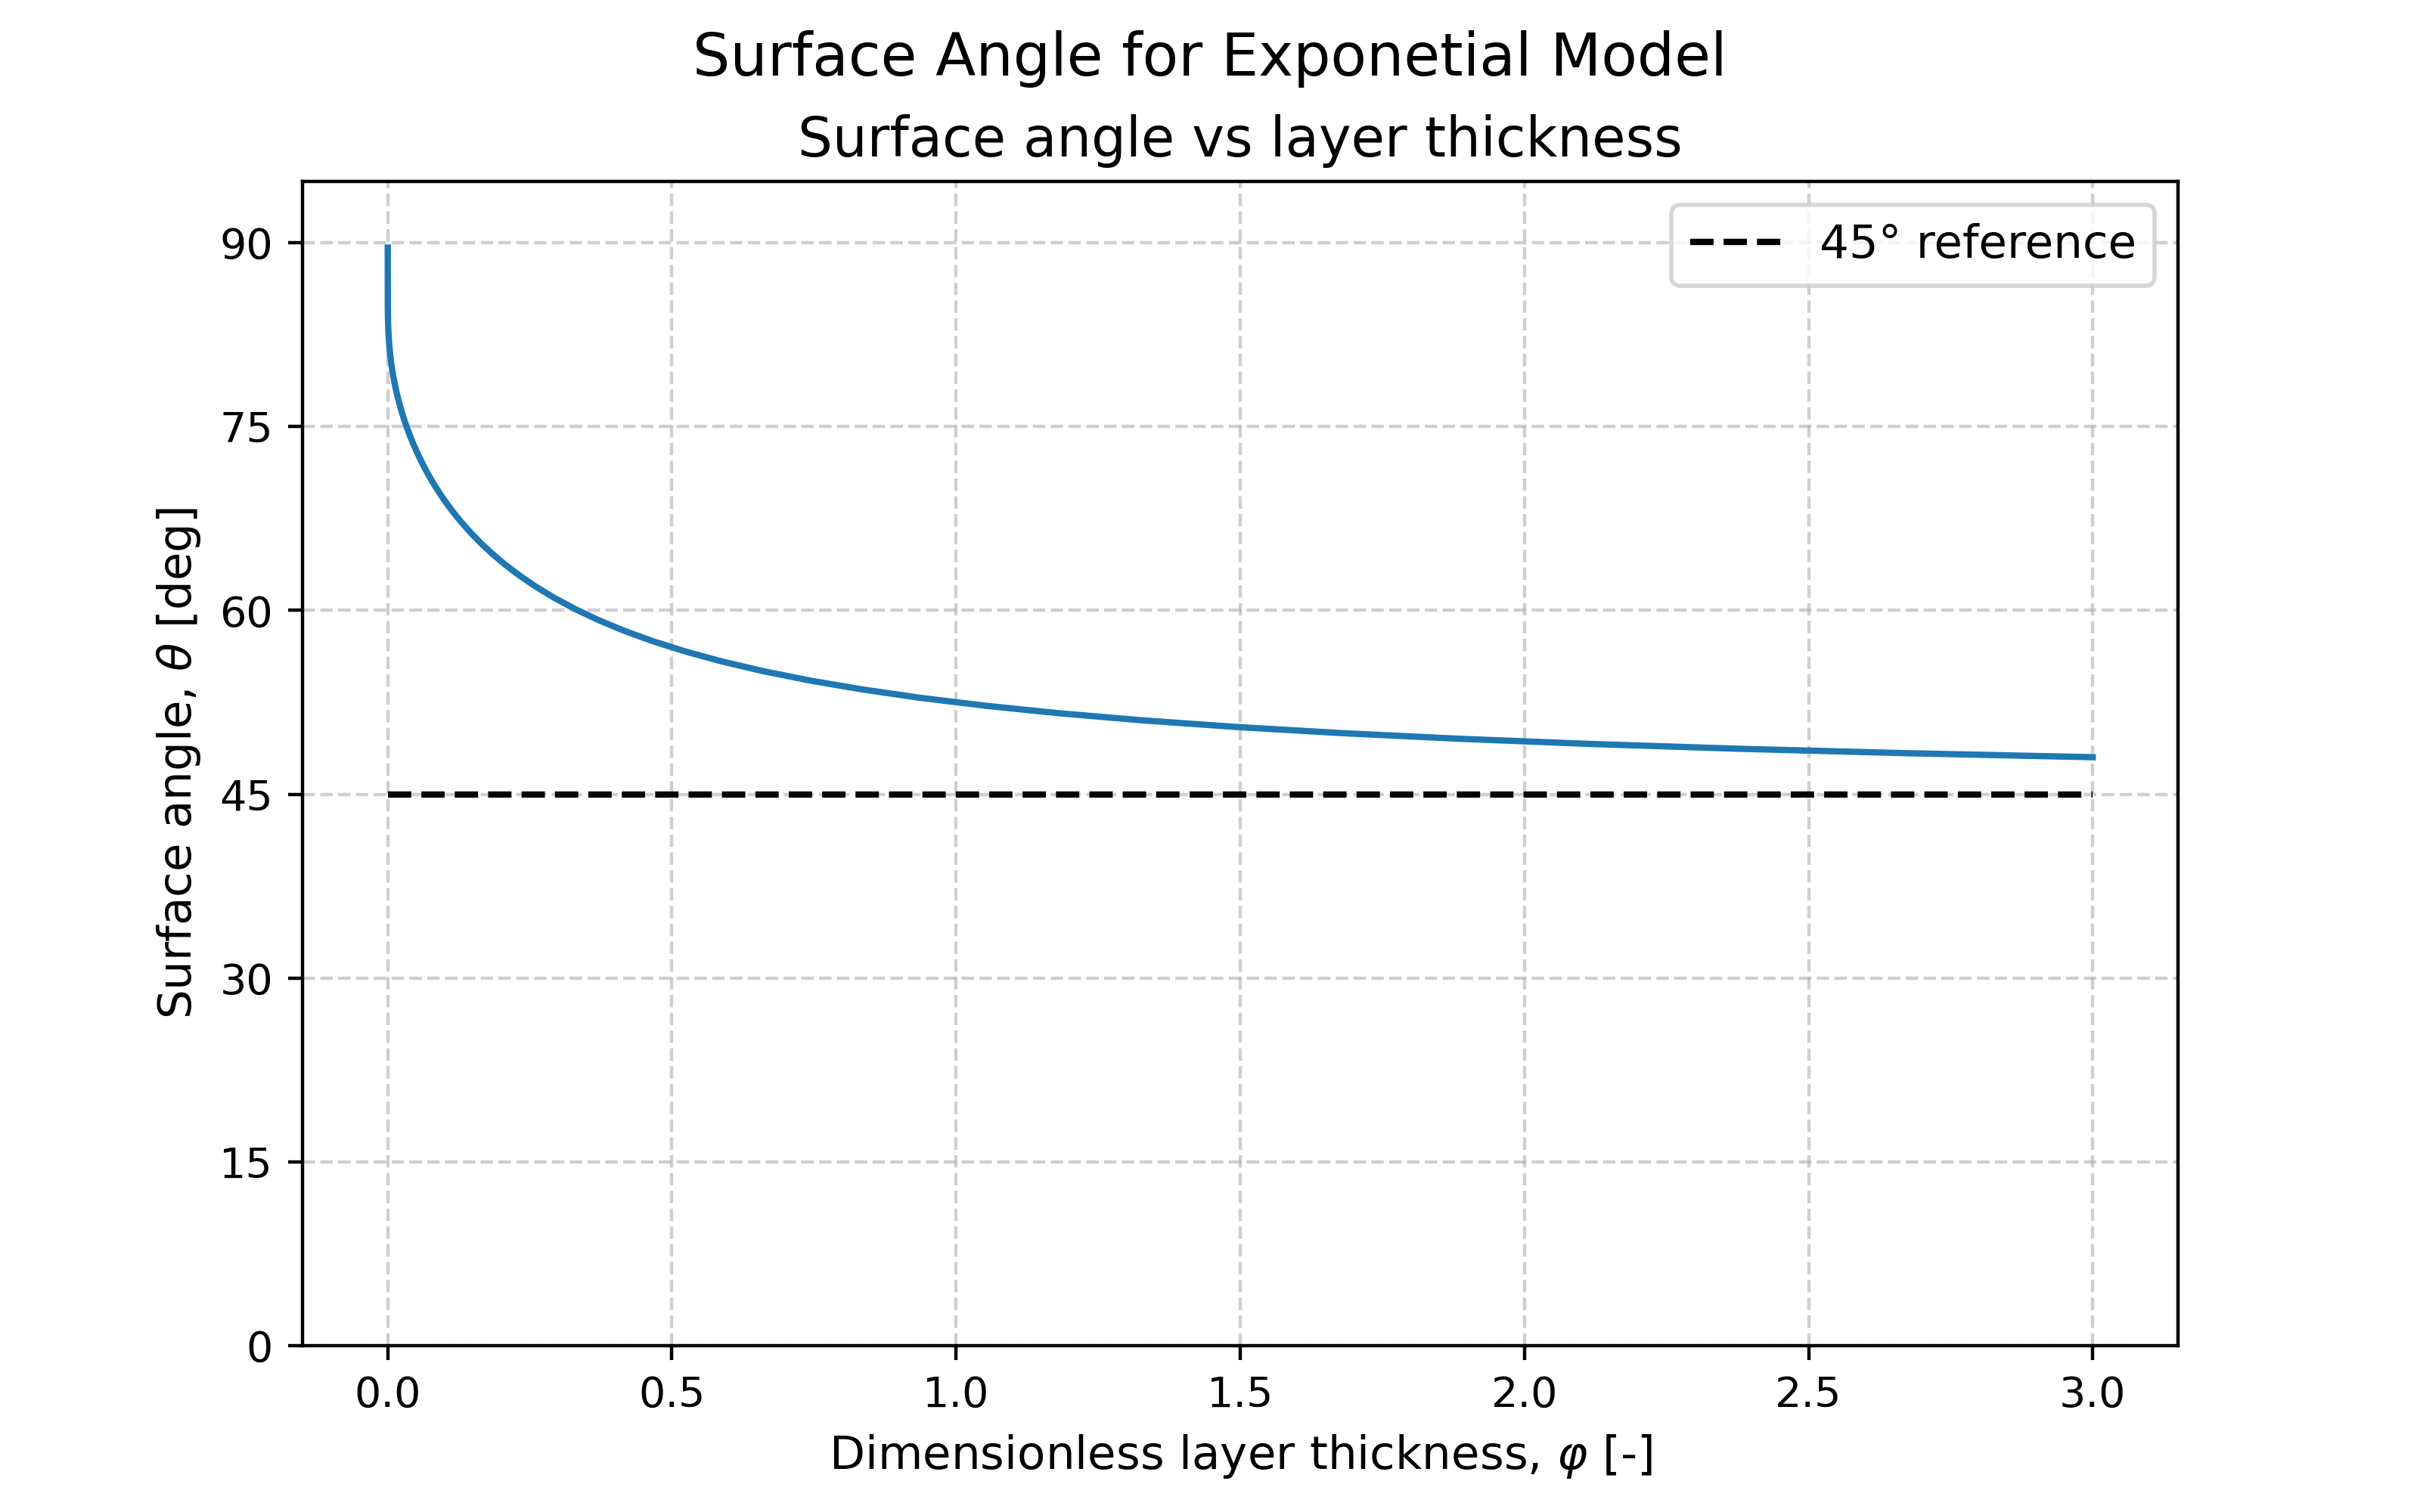
\includegraphics[height=0.37\textwidth]{Figures/exponential_angle.png}
    \caption{Surface angle for the exponentially decaying viscosity model as a function of the dimensionless parameter $\varphi$. The figure illustrates how vertical variations in eddy viscosity modify the classical Ekman turning angle.}
    \label{fig:exponential_angle}
\end{figure}

\subsection{The 1.5 model}

\begin{figure}[H]
    \centering    
    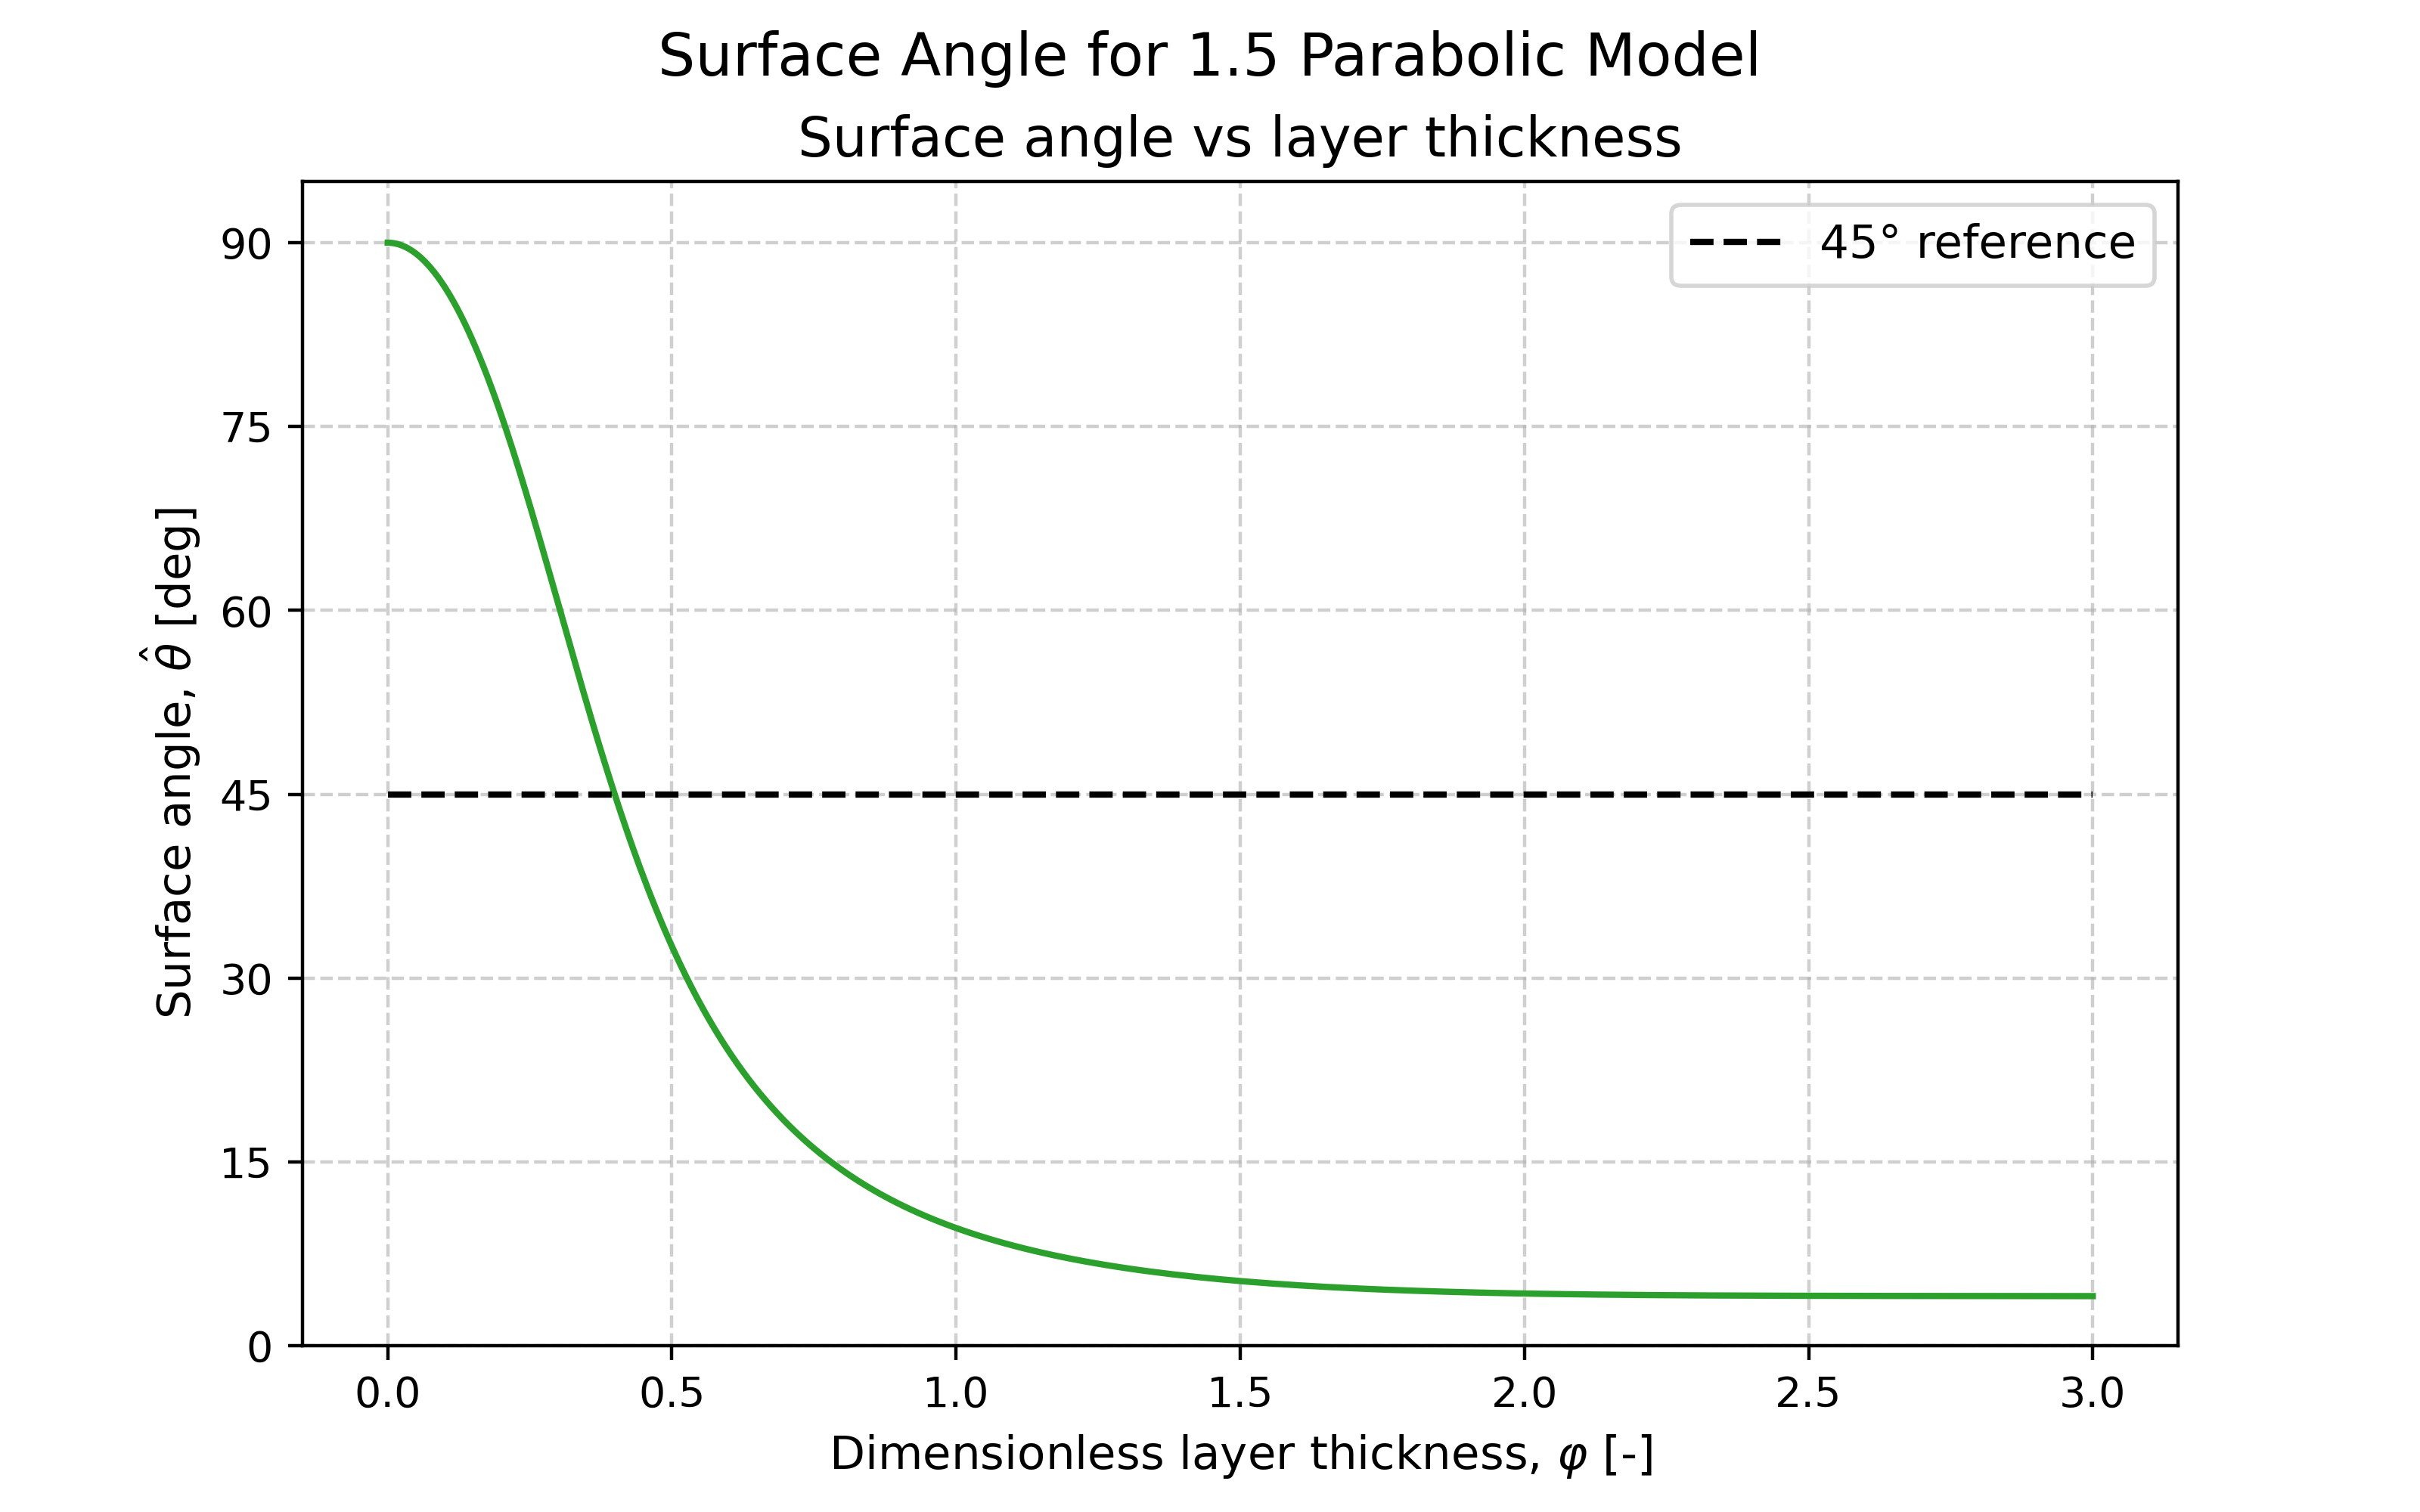
\includegraphics[height=0.37\textwidth]{Figures/numerical_15_parabolic_noramlized.png}
    \caption{Numerically computed surface angle for the parabolic viscosity profile in the 1.5-layer model. The angle is shown as a function of the normalized layer thickness for different maximum viscosities.}
    \label{fig:numerical_15_parabolic_noramlized}
\end{figure}

\begin{figure}[H]
    \centering    
    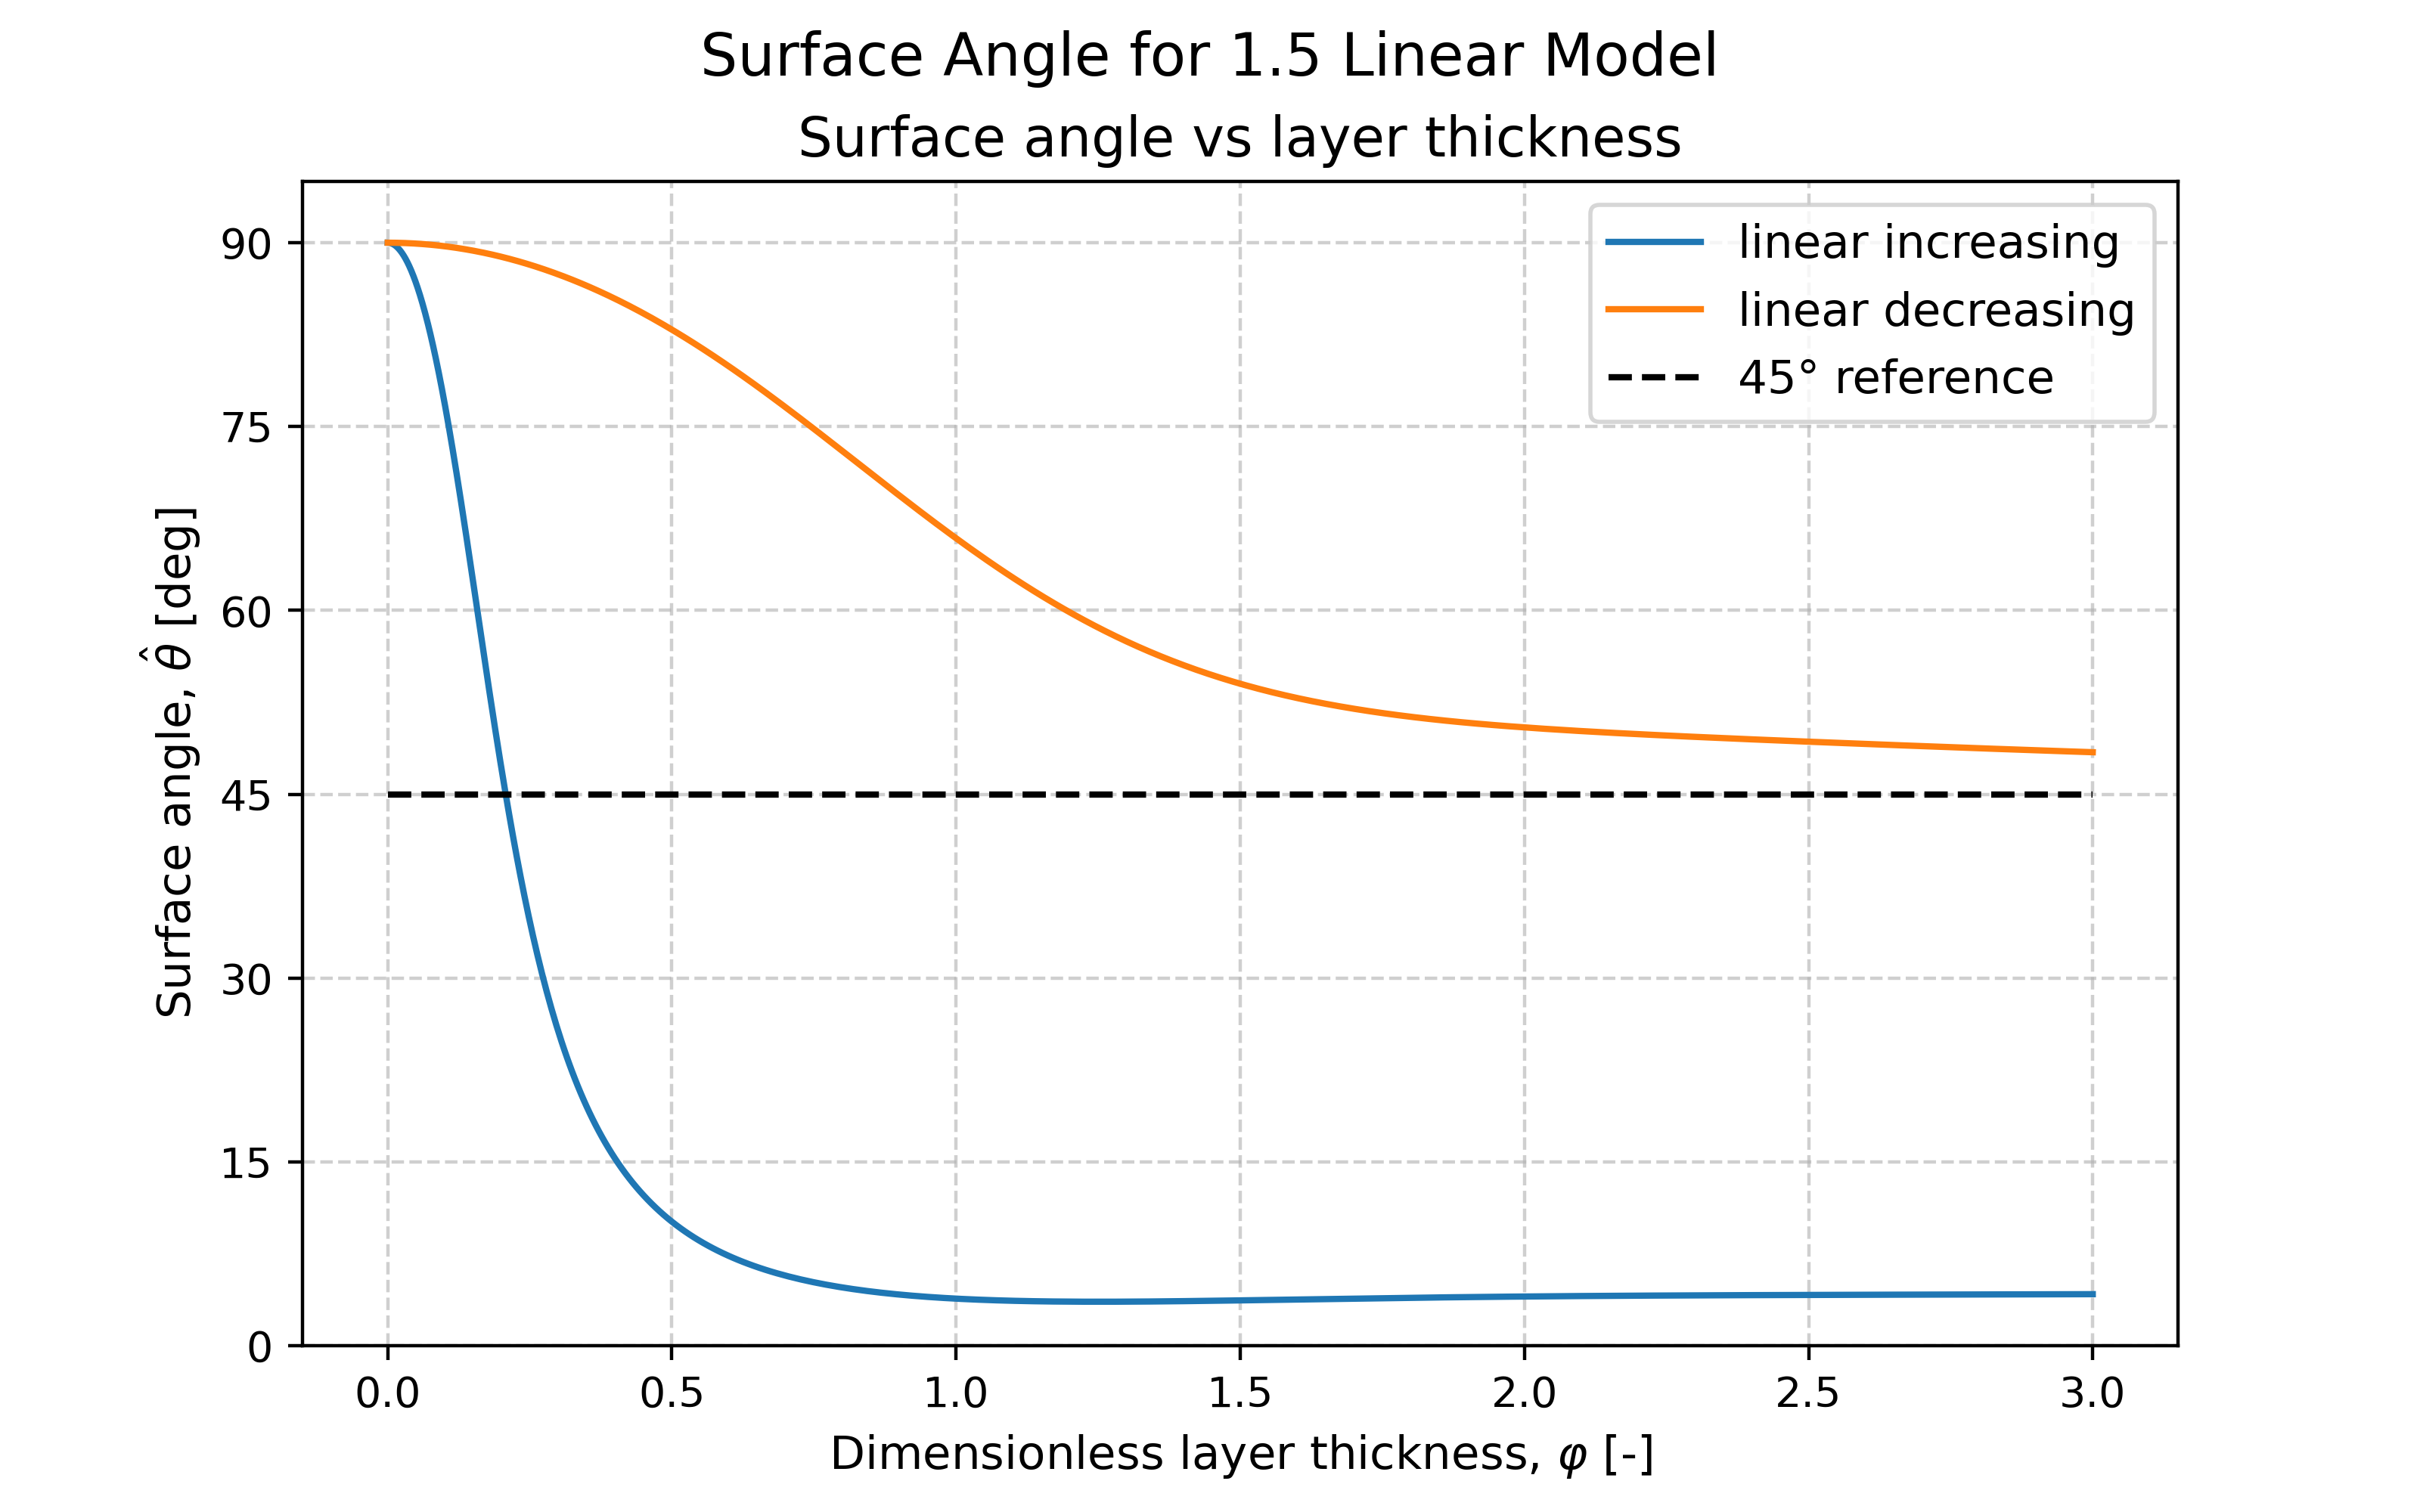
\includegraphics[height=0.37\textwidth]{Figures/numerical_15_linear_noramlized.png}
    \caption{Surface angle obtained numerically for linearly increasing and decreasing viscosity profiles in the 1.5-layer model. The results demonstrate how the vertical structure of viscosity affects the near-surface wind turning.}
    \label{fig:numerical_15_linear_noramlized}
\end{figure}